\section{Risikobewertung}


Die Risiken des Projektes sind in \acrshort{pren1} gesammelt und bewertet worden. Pro Risiko wurden Massnahmen zur Prävention und zur Mitigation gesammelt. Die Bewertung wurde durchgeführt vor dem Umsetzen der Massnahmen (V.) und nachher (N.).

Die Risiken sind in dieser Matrix auf Abbildung \ref{table:risk-table} ersichtlich vor und nach den Massnahmen.

\begin{table}[H]
\centering
\begin{subtable}{0.49\textwidth}
\centering
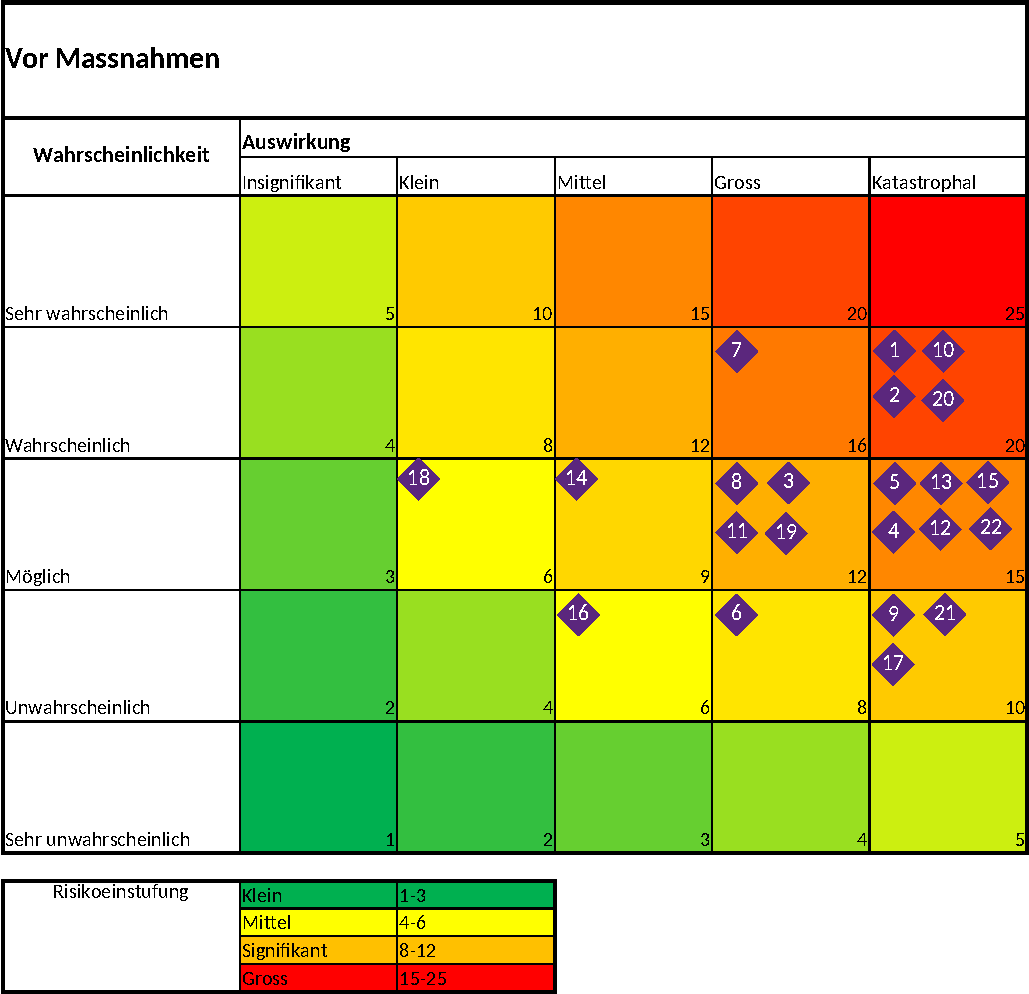
\includegraphics[width=0.99\linewidth]{assets/projektmanagement/Risikoanalyse_vorher-crop.pdf}
\caption{vor Massnahmen}
\label{table:risk-before}
\end{subtable}
\begin{subtable}{0.49\textwidth}
\centering
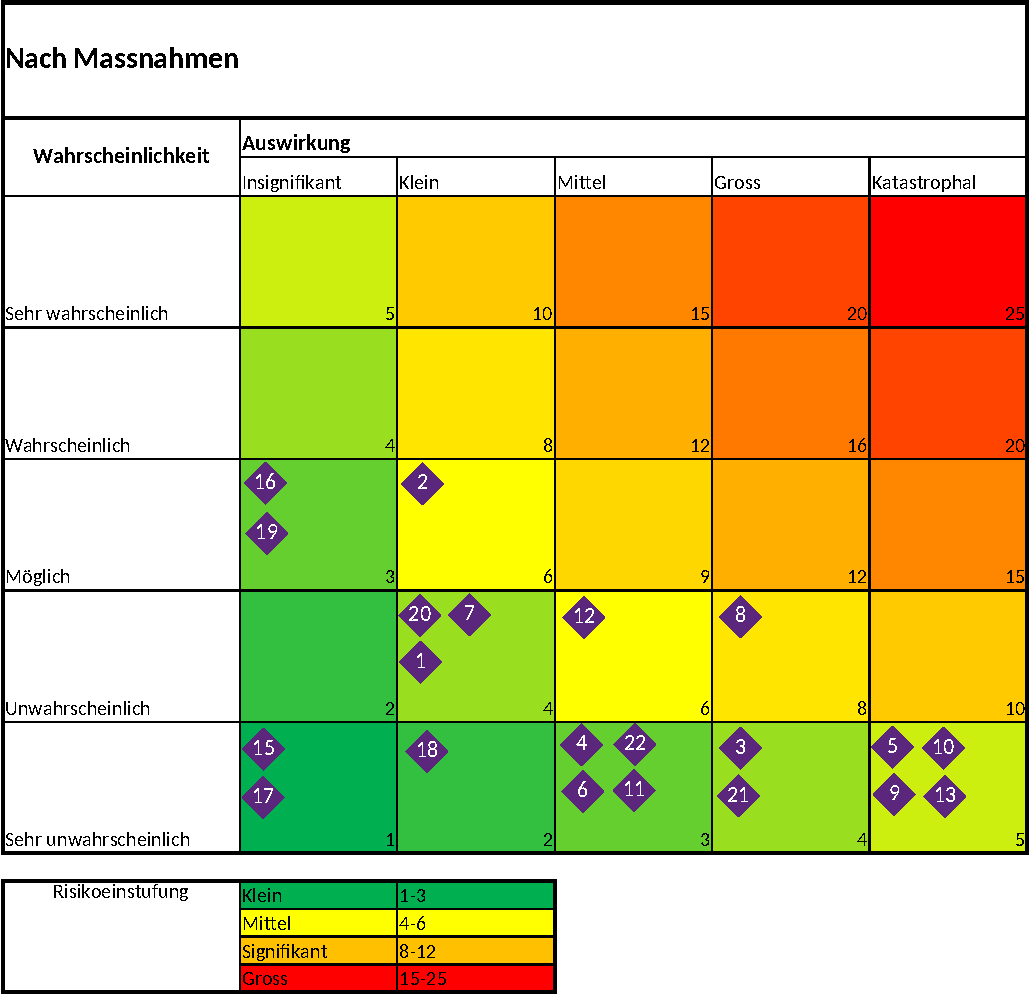
\includegraphics[width=0.99\linewidth]{assets/projektmanagement/Risikoanalyse_nachher-crop.pdf}
\caption{nach Massnahmen}
\label{table:risk-after}
\end{subtable}
\caption{Risikoanalyse}
\label{table:risk-table}
\end{table}

Aus der Risikomatrix nach den Massnahmen geht hervor, dass die grössten Risiken, die beim Entwickeln des Roboters berücksichtigt werden müssen, die folgenden drei sind:

\begin{itemize}
    \item Risiko 2: Knoten werden nicht erkannt.
    \item Risiko 8: Hindernisse werden beim Anheben verschoben.
    \item Risiko 12: Roboter wählt falschen Pfad.
\end{itemize}

Die folgende Tabelle \ref{table:risks} zeigt alle Risiken detailliert auf.  Jedes Risiko hat in dieser Arbeit neu eine weitere Kolonne "Ref.". Diese zeigt auf, in welchem Kapitel beschrieben wird, wie das Risiko behoben oder noch weiter mitigiert wurde, falls dies möglich war.

\begin{table}[H]
\centering
\small
\begin{tabularx}{\textwidth}{|c|X|X|X|c|c|c|}
\hline
  \textbf{Nr} & \textbf{Beschreibung} & \textbf{Prävention} & \textbf{Mitigation} & \textbf{V.} & \textbf{N.} & \textbf{Ref.}\\
  \hline
      1&Hindernisse werden nicht erkannt. &Mit vielen Bildern trainieren.& Distanzsensor erkennt Hindernisse, falls Bilderkennung nicht erkannt hat; Roboter fährt zurück, falls Distanzsensor erkennt.&20&4& \makecell{\ref{model-results}\\ \ref{ultraschall}} \\
  \hline
2&Knoten werden nicht erkannt. &Viele Bilder in verschiedenen Situationen machen, um zu trainieren.&Linien werden erkannt und Roboter orientiert sich daran.&20& 6&\ref{model-results}\\
  \hline
      3&4 Minuten reichen nicht. &Testdurchfläufe in realistischen Umgebungen.&&12&4 &\makecell{\ref{risks-sprint-2}\\ \ref{convert-yolo}}\\
  \hline
      4& 1 Minute reicht nicht zum Aufbau.& Testdurchfläufe und einfaches Interface.&Zufälliges Ziel wird gewählt von SW, falls bei Start keines ausgewählt.&15&3 &\ref{zieleingabe}\\
  \hline
      5&Bodenfugen werden als Linie erkannt. & Testdurchfläufe in realistischen Umgebungen.&Kamera hilft Linien zu erkennen, hilft Roboter gerade zu stellen.&15&5& \makecell{\ref{Liniensensor auslesen} \\ \ref{outgoing-lines}}\\
  \hline
      6& Liniensensor fehlerhaft. &Sichere Implementation mit Tests.& Encoder Motoren.&8&3 &\ref{Liniensensor auslesen}\\
  \hline
      7& Ein Objekt wird fälschlicherweise erkannt. &Knoten erkennen und nicht nur Hindernisse.&Roboter ist schnell genug, um Wege auszuprobieren und hat einen Trial \& Error Modus, der dies erlaubt.&16&4& \makecell{\ref{model-results} \\ \ref{navigation-arch}}
\\
  \hline
      8&Hindernisse werden beim Anheben verschoben. &Robuste Greifmethode wählen und testen.&&12&8& \\
  \hline
      9&Überstrom bei blockierten Motoren. &Endschalter, Stromsensoren.&Abschalten bevor Bauteile beschädigt.&10&5& \ref{motoren-encoder} \\
  \hline
      10&Ungenaue Abfahrtssituation vom Knoten, Fahrzeug fährt von der Linie weg. &Liniensensor als Unterstützung, Kamera prüft Linie& Falls keine Linie mehr erkannt, rückwärts fahren und korrigieren.&20&5& \ref{outgoing-lines}\\
  \hline
      11&Die Kamera liefert unscharfe oder verzerrte unbrauchbare Bilder. &Verwendung von Kameras mit hoher Auflösung.&Falls Bilder unscharf sind, Roboter anhalten und neue Bilder aufnehmen.&12&3&\ref{risks-sprint-1} \\
  \hline
        12& Der Roboter wählt einen falschen Pfad, da Objekte nicht erkannt werden. &Optimierung der Hinderniserkennung.& Falls Fehlzustand auftritt, kann Roboter zu vorherigen Knoten fahren und das vorher Gelernte zurücksetzen. Roboter ist schnell.&15& 6&\makecell{\ref{model-results} \\ \ref{ultraschall}\\ \ref{interface-nav-control}}\\
  \hline

\end{tabularx}
\end{table}

\newpage

\begin{table}[H]
\centering
\small
\begin{tabularx}\textwidth{|c | X | X | X | c | c|c|}
\hline
  \textbf{Nr} & \textbf{Beschreibung} & \textbf{Prävention} & \textbf{Mitigation} & \textbf{V.} & \textbf{N.} & \textbf{Ref.}\\
  
  \hline

        13&Ein Softwarefehler führt zu einem Absturz während der Laufzeit, wodurch der Roboter stoppt oder Fehlfunktionen aufweist. &Exception Handling und umfangreiche Tests unter verschiedenen Bedingungen.&Automatischer SW-Neustart, Wiederaufnahme des letzten bekannten Zustands.&15&5&\ref{risks-sprint-2} \\
  \hline
      14&Ein Software-Update führt zu neuen Fehlern oder ist nicht kompatibel mit der aktuellen Hardware. &Gründliche Tests vor dem Rollout eines Updates.& Durch SW-Versionierung hat man die Möglichkeit, schnell zur vorherigen stabilen Version zurückzukehren.&9&1&\ref{navigation-arch} \\
  \hline
      15&Akkustand ist zu niedrig bei Start des Laufes. & Anzeige des Akkustandes. Leicht austauschbarer Akku. Akku aufladen.&Ein zweiter Akku, der voll aufgeladen ist.&15& 1&\\
  \hline
      16&Personenausfall durch Krankheit oder Unfall. &&Stellvertretungen und virtuelle Kommunikation.&6& 3&-\\
  \hline
      17&Datenkorruption. &&Regelmässige Backups. Alle Dokumente auf Teams erstellen. Dokumentation in LaTeX auf Overleaf. Durch Cronjob werden jeden Tag die .tex Files auf GitHub gepusht.&10& 1&-\\
  \hline
  \multicolumn{7}{l}{Neue Risiken aus PREN 2} \\
  \hline
  18&Akkuhalterung geht kaputt & Akku vorsichtig austauschen. & Mehrere Akkuhalterungen erstellen. &6 &2&\ref{Batteriefach konstruieren}\\
  \hline
  19&Elektronische Komponent geht kaputt & Vorsichtig damit umgehen und nicht unnötig anfassen. & Mehrere Exemplare bereithalten. &12 &3&\ref{pcb}\\
  \hline
    20&Robtoter weiss nicht mehr wo er sich befindet.& Robuste Bilderkennung und Wegfindungsmethode. & Trial \& Error Modus implementieren. &20&4&\ref{navigation-arch}\\
  \hline
    21&Ausgehende Linien werden nicht erkannt. & Objekterkennung testen. & Aus anderer Distanz noch einmal versuchen und falls immer noch nicht erkannt, Knoten aus internem Graph entfernen. & 10&4&\ref{outgoing-lines}\\
  \hline
      22&Gibt fälschlich am Ziel zu sein oder erkennt Ziel nicht. & Robuste Methode, um Graph zu traversieren und sich zu merken, wo man ist. & Methode um Buchstaben auf Knoten zu erkennen implementieren. & 15&3&\ref{detect-target}\\
  \hline

\end{tabularx}
\caption{Risiken}
\label{table:risks}
\end{table}
